\documentclass[a4paper]{article}
\usepackage{tikz}
\usetikzlibrary{positioning,calc}
\begin{document}
\pagestyle{empty}
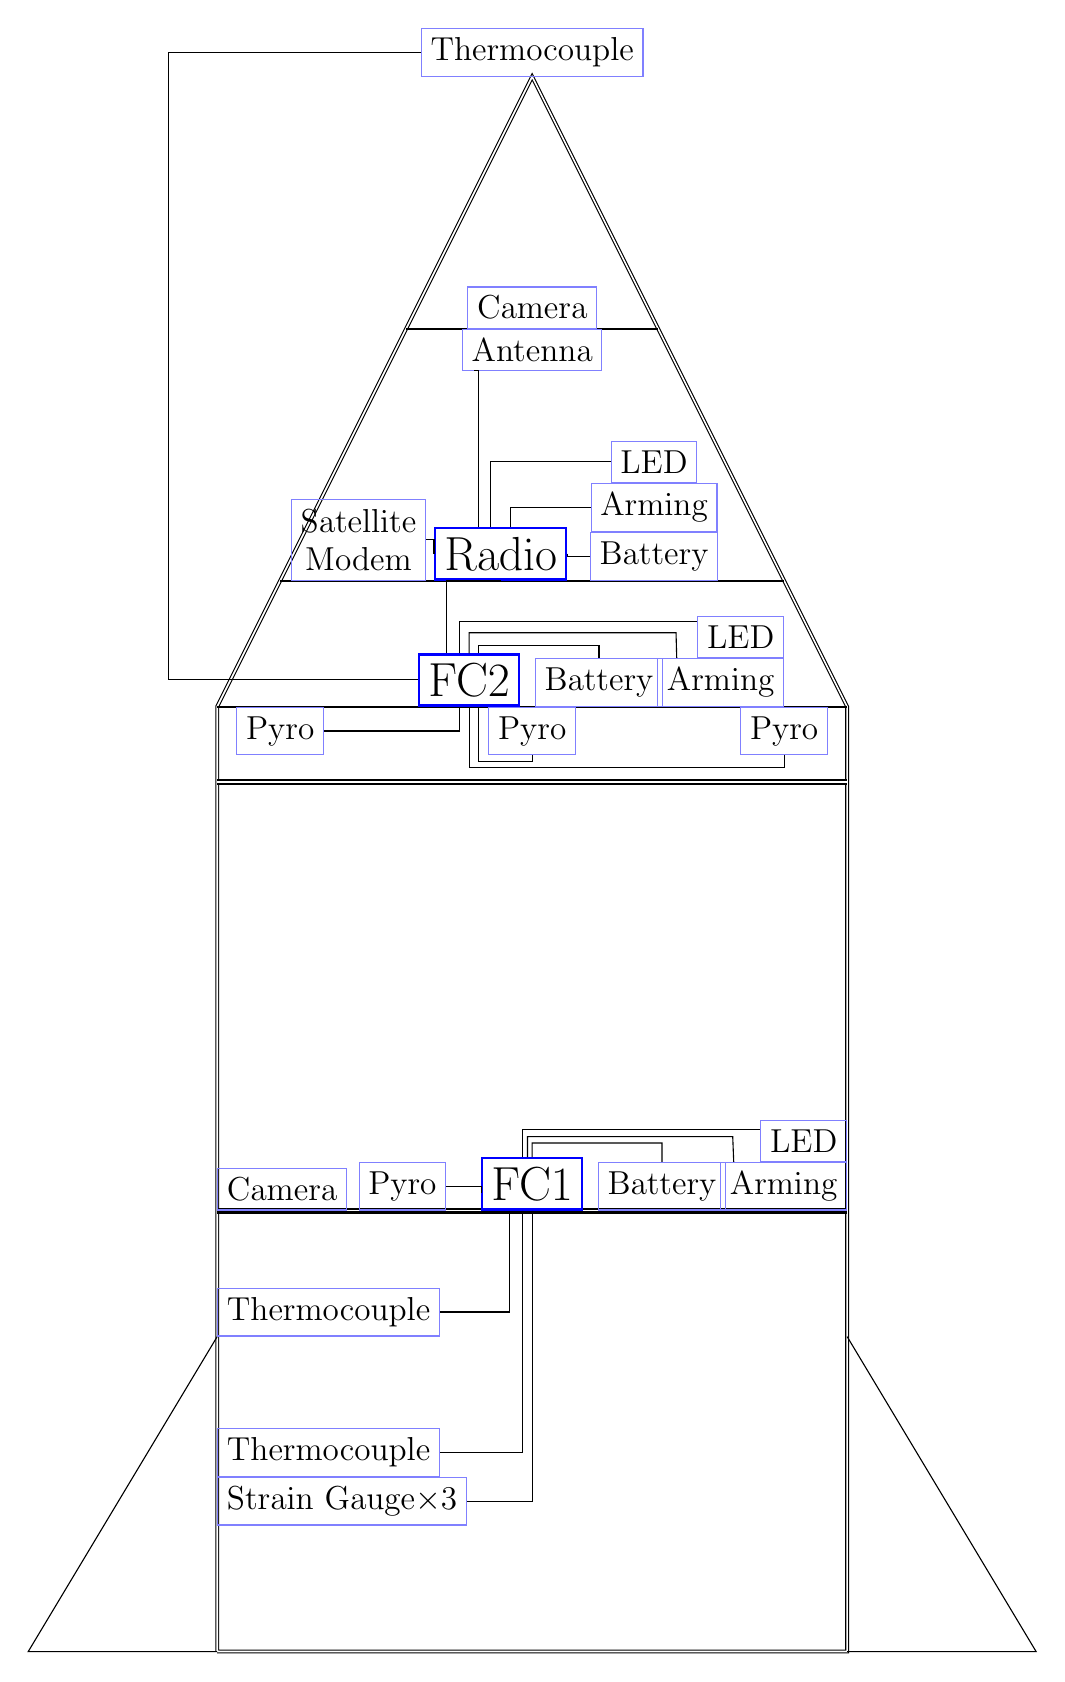
\begin{tikzpicture}
    [scale=0.8,
     master/.style={draw=blue!100,thick,anchor=south,font=\LARGE},
     slave/.style={draw=blue!50,anchor=south,font=\large}]
    % Body
    \draw [double] (0, 0) -- (0, 15) -- (5, 25) -- (10, 15) -- (10, 0) -- (0, 0);

    % Fins
    \draw (0, 0) -- (-3, 0) -- (0, 5);
    \draw (10, 0) -- (13, 0) -- (10, 5);

    % Mounting Plates
    \draw [thick,double] (0, 7) -- (10, 7);
    \draw [thick,double] (0, 13.8) -- (10, 13.8);
    \draw [thick] (0, 15) -- (10, 15);
    \draw [thick] (1, 17) -- (9, 17);
    \draw [thick] (3, 21) -- (7, 21);

    % Main Body
    \node (fc1) at (5, 7) [master] {FC1};
    \node (fc1bat) [right=1 of fc1.south east] [slave] {Battery};
    \node (fc1arm) at (10, 7) [slave, anchor=south east] {Arming};
    \node (fc1led) [above=0 of fc1arm.north east] [slave, anchor=south east] {LED};
    \node (fc1pyro) [left=1 of fc1.south west] [slave] {Pyro};
    \node (fc1sg) at (0, 2) [slave, anchor=south west] {Strain Gauge$\times3$};
    \node (fc1tc1) [above=0 of fc1sg.north west] [slave, anchor=south west] {Thermocouple};
    \node (fc1tc2) at (0, 5) [slave, anchor=south west] {Thermocouple};
    \node (bcam) at (0, 7) [slave,anchor=south west] {Camera};

    \draw (fc1.190) |- (fc1pyro);
    \draw (fc1.110) |- (fc1led.165);
    \draw (fc1.100) |- ($(fc1arm.north west) + (0.2, 0.4)$) -- (fc1arm.154);
    \draw (fc1.90)  |- ($(fc1bat.north) + (0, 0.3)$) -- (fc1bat);
    \draw (fc1.230) |- (fc1tc2);
    \draw (fc1.250) |- (fc1tc1);
    \draw (fc1.270) |- (fc1sg);

    % Nosecone Base
    \node (fc2) at (4, 15) [master] {FC2};
    \node (fc2bat) [right=1 of fc2.south east] [slave] {Battery};
    \node (fc2arm) at (9, 15) [slave, anchor=south east] {Arming};
    \node (fc2led) [above=0 of fc2arm.north east] [slave, anchor=south east] {LED};
    \node (fc2pyro1) at (1, 15) [slave, anchor=north] {Pyro};
    \node (fc2pyro2) at (5, 15) [slave, anchor=north] {Pyro};
    \node (fc2pyro3) at (9, 15) [slave, anchor=north] {Pyro};

    \node (r) at (4.5, 17) [master] {Radio};
    \node (rbat) [right=1.1 of r.south east] [slave] {Battery};
    \node (rarm) [above=0 of rbat.north] [slave] {Arming};
    \node (rled) [above=0 of rarm.north] [slave] {LED};
    \node (rant) at (5, 21) [slave,anchor=north] {Antenna};
    \node (rb) [left=0.1 of r.south west] [slave,anchor=south east,align=center]
    {Satellite\\Modem};

    \node (ncam) at (5, 21) [slave,anchor=south] {Camera};
    \node (ntc) at (5, 25) [slave,anchor=south] {Thermocouple};

    \draw (fc2.250) |- (fc2pyro1);
    \draw (fc2.270) |- ($(fc2pyro3.south) - (0, 0.2)$) -- (fc2pyro3.south);
    \draw (fc2.290) |- ($(fc2pyro2.south) - (0, 0.1)$) -- (fc2pyro2.south);

    \draw (fc2.110) |- ($(fc2led.north west) - (0, 0.1)$);
    \draw (fc2.90)  |- ($(fc2arm.north west) + (0.3, 0.4)$) -- (fc2arm.151);
    \draw (fc2.70)  |- ($(fc2bat.north) + (0, 0.2)$) -- (fc2bat.north);
    \draw (fc2.130) |- (r.south);
    \draw (fc2.180) -| ($(ntc.west) - (4, 0)$) -- (ntc.west);

    \draw (r.east) |- (rbat.west);
    \draw (r.70) |- (rarm.west);
    \draw (r.110) |- (rled.west);
    \draw (r.130) |- (rant.200);
    \draw (r.west) |- (rb.east);
\end{tikzpicture}
\end{document}
